\section{Grover's Algorithm}
Grover's algorithm can be used to speed up the SAT problem. \\
Let
$$f: \binset^n \to \binset$$
we restrict it to
$$\begin{cases}
    f(\mathbf{x}) = 0 & \forall \mathbf{x} \in \binset^n \\
    f(\mathbf{x}) = 0 & \exists! \mathbf{x}^* \in \binset^n, f(\mathbf{x}^*) = 1
\end{cases}$$
The quantum circuit for Grover's algorithm is the following:
\begin{center}
    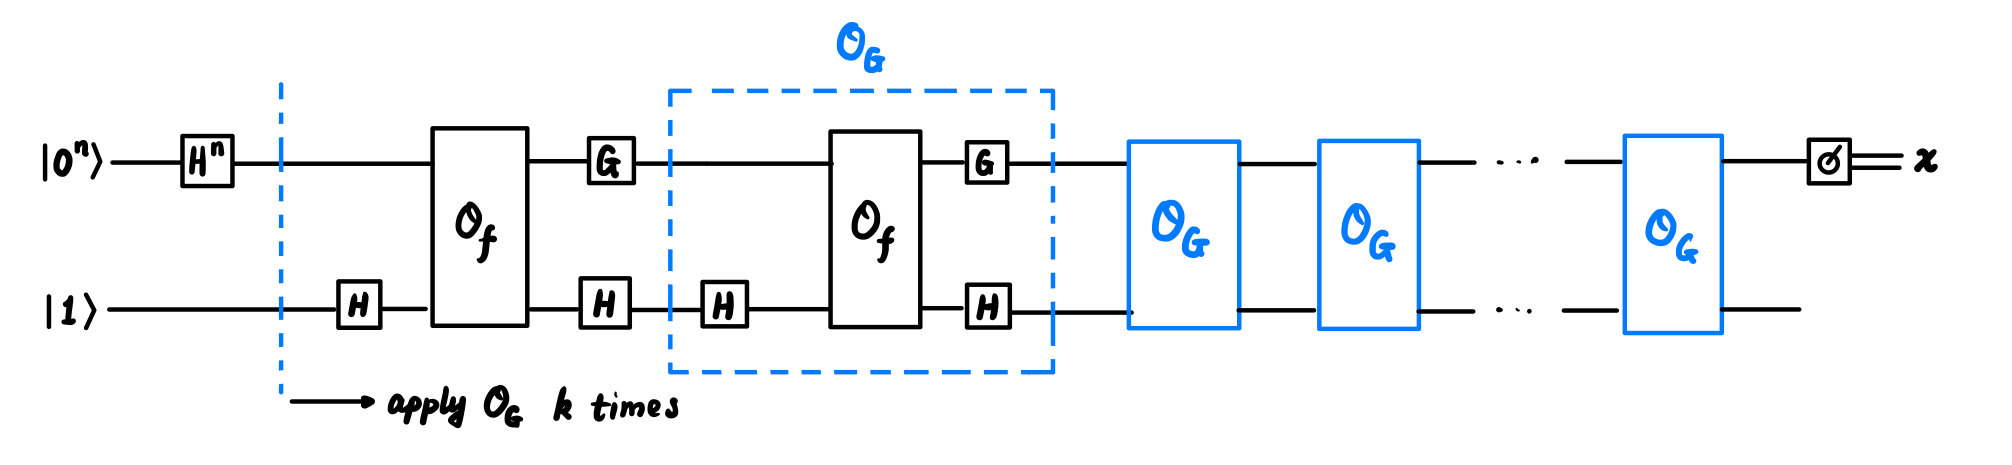
\includegraphics[scale = 0.2]{9/grover.png}
\end{center}
Recall the quantum phase oracle for $f$ is
$$\opuni_f = HO_fH: \ket{\mathbf{x}} \ket{b} \mapsto (-1)^{b \cdot f(\mathbf{x})} \ket{\mathbf{x}}\ket{b}$$
We define $V_f$ where (take $b = 1$ for $\opuni_f$)
$$V_f: \ket{\mathbf{x}} \mapsto (-1)^{f(\mathbf{x})}\ket{\mathbf{x}}$$
and define:
$$\ketpsi = \frac{1}{\sqrt{2^n}}\Sumi{\mathbf{x}}\ket{\mathbf{x}}$$
$$G := \id - 2\op{\psi}$$
The state before measurment in this setup is essentially
$$(GV_f)^kH^n\ket{0^n}$$
In the first case, this becomes $(-1)^k \ketpsi$. \\
In the second case, $\ketpsi$ can be written as:
$$\ketpsi = \sqrt{\frac{N - 1}{N}} \ket{\psi_0} + \sqrt{\frac{1}{N}} \ket{\psi_1} = \cos \theta \ket{\psi_0} + \sin \theta \ket{\psi_1}$$
where $N = 2^n$, and
$$\ket{\psi_{0}} = \frac{1}{\sqrt{N -1}} \Sumi{\mathbf{x} \ne \mathbf{x}^*} \ket{\mathbf{x}}$$
$$\ket{\psi_1} = \ket{\mathbf{x}^*}$$
We can calculate $-GV_f$ with respect to $\ket{\psi_0}$ and $\ket{\psi_1}$ to be:
$$\begin{pmatrix}
    \cos 2\theta & -\sin 2\theta \\
    \sin 2\theta & \cos 2\theta
\end{pmatrix}$$
which is rotating $2 \theta$ counterclockwise. \\
In the second case, $\ketpsi$ starts with a $\theta$ between it and the $\ket{\psi_0}$ axis, and after applying $-GV_f$ $k$ times, we want it to be close to $\ket{\psi_1}$. This means:
$$(2k + 1)\theta = \frac{\pi}{2} \to k \approx \frac{\pi}{4}\sqrt{N}$$
(Soufflé problem: fixed point amplification)

\subsection{Limitations of Quantum Algorithm in Query Models}
We demonstrate that if a quantum computer can only query $f$, it must use $\Omega(\sqrt{2^n})$ queries to decide if $f$ maps $\mathbf{x}$ to $1$. \\
We consider a general model of any quantum algorithm:
\begin{center}
    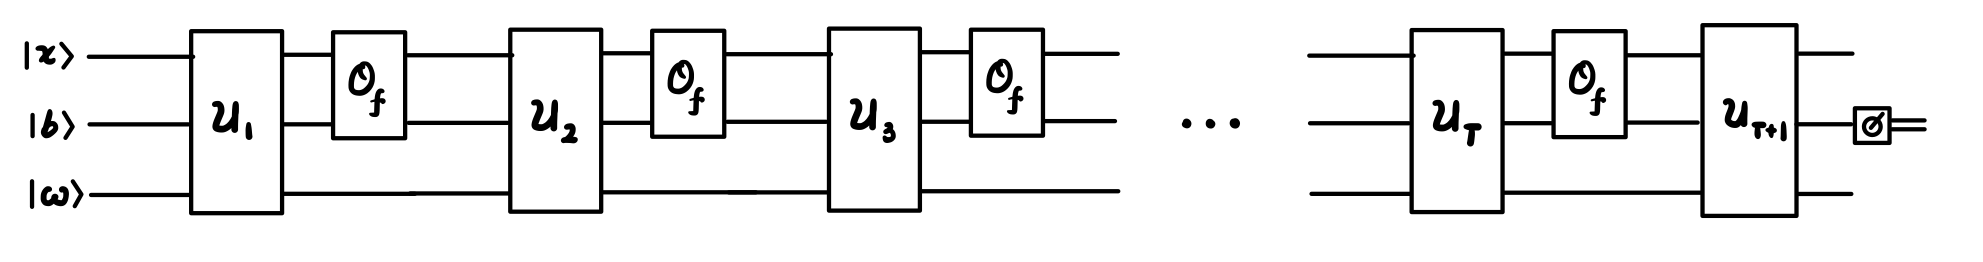
\includegraphics[scale = 0.2]{9/general_qc.png}
\end{center}
Here, $T$ represents the number of queries to $f$. \\
We consider the circuit for different choices of $f$, denote the circuit where $f$ maps everything to $0$ to be ``0'', $f$ maps $\mathbf{x}_i$ to $1$ and the rest to $0$ to be ``$\mathbf{x}_i$''. \\
The limitation is that if $T$ is small, the algorithm can ``look at'' at most $T^2$ values of $f(\mathbf{x})$, and if $T^2 < N$, there will exist $\mathbf{x}^* \ne \mathbf{x}_i$ such that the output of circuit ``0'' is indistinguishable from ``$\mathbf{x}^*$''.
\begin{center}
    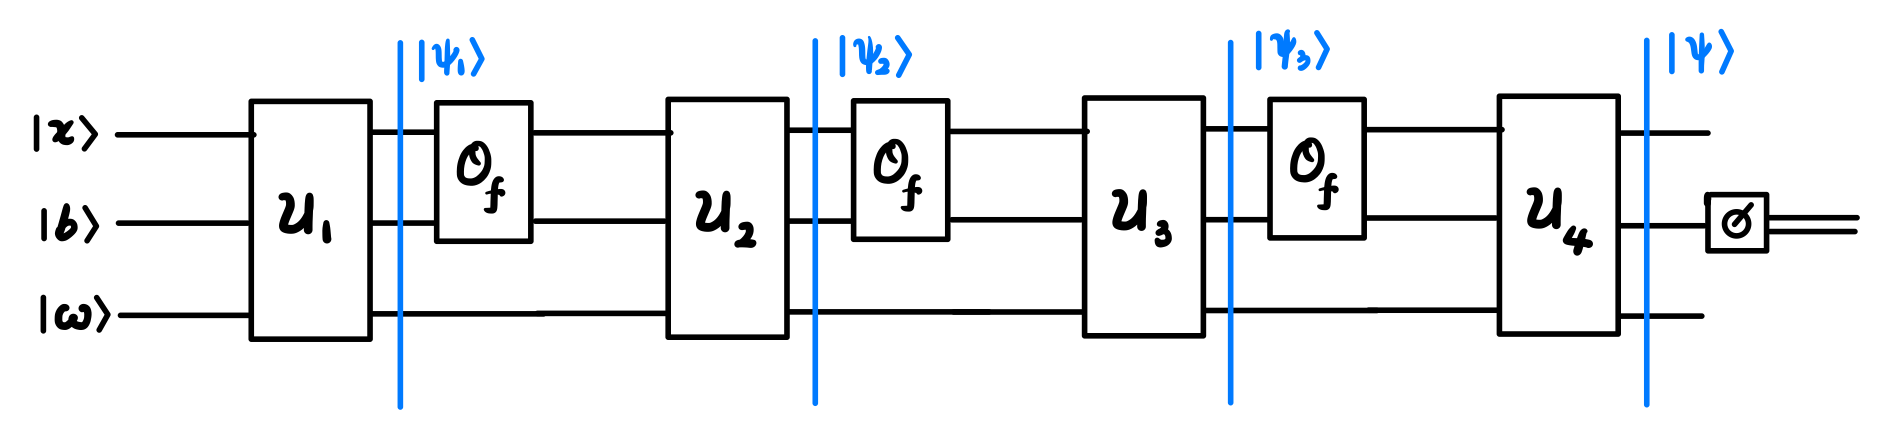
\includegraphics[scale = 0.2]{9/3-step.png}
\end{center}
Let $t \in \{1, \dots, T\}$ and $\ket{\psi_t}$ be the state for $t$th query, we write:
$$\ket{\psi_t} = \Sumi{\mathbf{x}, b, \omega} \alpha_{\mathbf{x}, b, \omega}^t \ket{\mathbf{x}, b, \omega}$$
where $t$ is just a \textbf{superscript}. \\
Let
$$Q_\mathbf{x}^t = \Sumi{b, \omega} \abs{\alpha_{\mathbf{x}, b, \omega}^t}^2$$
$$Q_\mathbf{x} = \Sum{t = 1}{T} Q_\mathbf{x}^t$$
Then, by expanding the terms:
$$\Sumi{\mathbf{x}}Q_\mathbf{x} = T$$
there must exist $x^*$ such that $Q_{\mathbf{x}^*} \le \frac{T}{N}$. This means, if $T < \sqrt{N}$, the quantum circuit cannot distinguish circuit ``0'' from circuit ``$\mathbf{x}^*$''. \\
We show this by considering a function, $g: \binset^n \to \binset$ such that $g(\mathbf{x}^*) = 1$ and $g(\mathbf{x}) = 0$ for $\mathbf{x} \ne \mathbf{x}^*$.
\begin{theorem}
    Let $\ket{\gamma}$ be the state of circuit ``$\mathbf{x}$'' just before measurement, Then
    $$\norm{\ketpsi - \ket{\gamma}} \le 2 \Sum{t = 1}{T} \sqrt{Q_{\mathbf{x}^*}^t}$$
\end{theorem}
The idea behind this is that we first replace the last $f$ from circuit ``0'' with $g$ and bound the difference. Then replace the last two $f$ from circuit ``0'' with $g$ and bound the difference. Eventually, we replace all $f$ with $g$ and bound the difference.
\begin{theorem}
    At time step $t$, we replace the last $T - t + 1$ $f$ with $g$, and we can show that at each replacement, the difference between states just before measurement is bound by $4Q_{\vecx}^t$
\end{theorem}
Then:
\begin{align*}
    \norm{\ketpsi - \ket{\gamma}} &\le 2 \Sum{t = 1}{T} \sqrt{Q_\vecx^t} \\
    &= 2 \Sum{t = 1}{T} 1 \cdot \sqrt{Q_\vecx^t} \\
    &\le 2 \sqrt{T} \sqrt{\Sum{t = 1}{T} Q_\vecx^t} \\
    &= \frac{2T}{\sqrt{N}}
\end{align*}
which is small unless $T \ge \Omega(\sqrt{N})$.

\newpage